\section{Introduction}

Autonomous driving is a control problem in which a vehicle must identify the drivable region, avoid obstacles, keep a coherent direction of motion and reach a target. This project studies this problem through a 2D simulator and a reinforcement learning controller supported by a Kohonen self-organizing map.

The application consists of a rectangular car moving on user-defined tracks. Each track has a start line, a finish line, road borders and optional circular obstacles. The vehicle observes the environment through lidar-like distance sensors and chooses discrete actions that modify its acceleration and heading. The objective is to reach the finish line while avoiding collisions with both borders and obstacles, and while keeping the trajectory reasonably efficient.
The central idea is to combine two learning components. A self-organizing map (SOM), also known as a Kohonen map, discretizes continuous lidar measurements into a finite state index. A tabular Q-learning agent then learns an action value for each discrete state-action pair.

The project was implemented in Python using modular components for track creation, environment simulation, SOM training, reinforcement learning training, inference and quantitative evaluation. The final workflow supports both interactive visual inspection through Pygame and batch evaluation over a collection of test tracks. An example of the system in action is shown in \Cref{fig:example}: the car (yellow rectangle) is navigating a track with borders (grey lines) and obstacles (red circles); the lidar sensors are represented as blue rays, and the target finish line is shown in yellow.

The report is organized as follows. \Cref{ch:overview} introduces the system architecture and the main specifications. \Cref{ch:implementation} describes the simulator, the SOM and the Q-learning algorithm. \Cref{ch:evaluation} defines the evaluation metrics and presents the generated analysis plots. Finally, \Cref{ch:conclusions} summarizes the achieved results and discusses possible extensions.

\begin{figure}[ht]
    \centering
    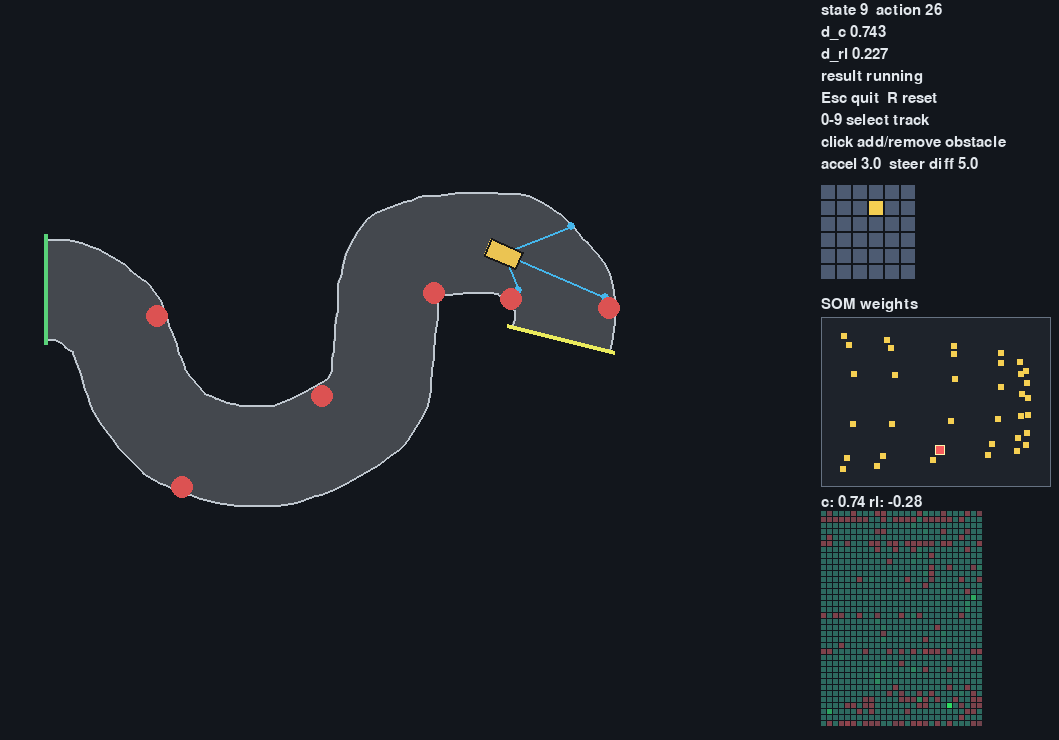
\includegraphics[width=0.7\textwidth]{images/1/screen.png}
    \caption{An example of the system in action.}
    \label{fig:example}
\end{figure}
